\documentclass[tikz,border=3mm,multi=tikzpicture]{standalone}
\usepackage[utf8]{inputenc}
\usepackage[T1]{fontenc}
\usepackage{helvet}
\renewcommand{\familydefault}{\sfdefault}
\usepackage{tikz}
\usetikzlibrary{positioning}
\begin{document}

\tikzset{every node/.append style={font=\sffamily\small}}
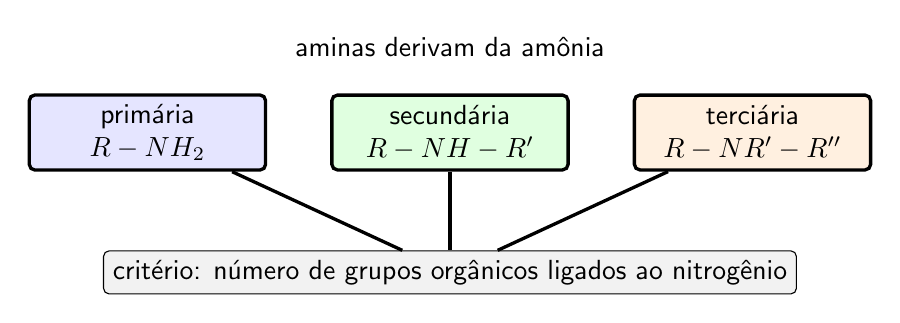
\begin{tikzpicture}[node distance=0.8cm]
  \tikzstyle{box}=[draw,rounded corners=2pt,very thick,minimum width=3cm,minimum height=0.95cm,align=center]
  \node[box,fill=blue!10] (a1) {primária\\$R-NH_2$};
  \node[box,fill=green!12,right=0.8cm of a1] (a2) {secundária\\$R-NH-R'$};
  \node[box,fill=orange!12,right=0.8cm of a2] (a3) {terciária\\$R-NR'-R''$};
  \node[draw,rounded corners=2pt,fill=gray!10,align=center,below=1cm of a2] (n) {critério: número de grupos orgânicos ligados ao nitrogênio};
  \draw[very thick] (a1) -- (n);
  \draw[very thick] (a2) -- (n);
  \draw[very thick] (a3) -- (n);
  \node[align=center,above=0.35cm of a2] {aminas derivam da amônia};
\end{tikzpicture}

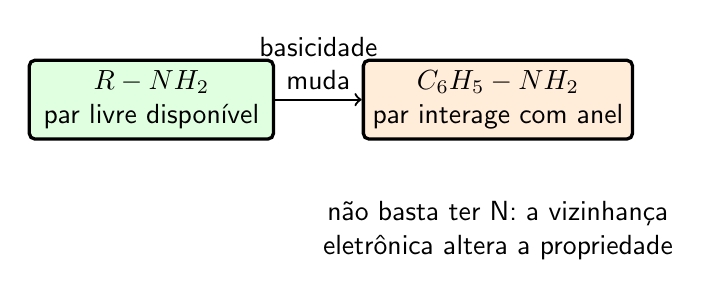
\begin{tikzpicture}[node distance=0.9cm]
  \tikzstyle{box}=[draw,rounded corners=2pt,very thick,minimum width=3.1cm,minimum height=1.0cm,align=center]
  \node[box,fill=green!12] (alif) {$R-NH_2$\\par livre disponível};
  \node[box,fill=orange!15,right=1.1cm of alif] (anil) {$C_6H_5-NH_2$\\par interage com anel};
  \draw[->,thick] (alif) -- node[above,align=center] {basicidade\\muda} (anil);
  \node[align=center,below=0.65cm of anil] {não basta ter N: a vizinhança\\eletrônica altera a propriedade};
\end{tikzpicture}
\end{document}
